\documentclass[11pt, a4paper]{article}

%\usepackage[T1]{fontenc}
%\usepackage{fullpage}

\usepackage[utf8]{inputenc} % comment when using lualatex
\usepackage[italian]{babel} % lingua e a-capo-sillabato
\usepackage{graphicx}
\usepackage[hidelinks]{hyperref} % link di pagina
\usepackage[bottom]{footmisc} % note appiccicate al fondo della pagina
\usepackage{float} % per posizionamento immagini
\usepackage{amsthm} % per ambienti stile teorema
\usepackage{tabularx} %tabelle
\usepackage[table]{xcolor} %colore caselle
\usepackage{enumitem} %additional commands for lists

\usepackage{fancyhdr}
\pagestyle{fancy}
\fancyhf{}% Clear header/footer
\fancyhead[C]{\footnotesize\textit{Documento:} D2 \hfill SleepCode \hfill \textit{Versione:} 1.0}
\renewcommand{\headrule}{{\color{red!70}\rule{\textwidth}{2pt}}}


%\pagestyle{myheadings}
%\markright{John Smith\hfill On page styles\hfill}

\renewcommand\UrlFont{\color{blue}\rmfamily}

\theoremstyle{definition}

\newtheorem{funcreq}{RF} %% numerazione dei requisiti funzionali
\newtheorem{nonfuncreq}{RNF} %% requisiti non funzionali
\newtheorem{backend}{BE}
\newtheorem{frontend}{FE}

\title{Specifica dei Requisiti}

\author{Raffaele \textsc{Castagna}\\
Alberto \textsc{Rovesti}\\
Zeno \textsc{Saletti}}

\newcommand{\groupNumber}{G17}


% —

% Web address for the project (if any)
% \newcommand{\homepage}{\url{https://www.}}


% data
\date{\today}

\makeatletter{}

% IL PREAMBOLO FINISCE QUI %%%%%%%%%%%%%%%%%%%%%%%%%%%%%%%%%%%%%%%%%%%%%%%%%%%%






\begin{document}

% La pagina di copertina si trova in un file .tex a parte
% NON MODIFICARE QUESTO COMANDO!!!
\begin{titlepage}
\newcommand{\HRule}{\rule{\linewidth}{0.3mm}} % Defines a new command for horizontal lines, change thickness here
\center % Centre everything on the page

%------------------------------------------------
%	Logo
%------------------------------------------------

\includegraphics[width=0.3\textwidth]{materiale/UniTrento_logo_ITA_colore.png}\\[0.5cm]
%------------------------------------------------
%	Headings
%------------------------------------------------
\textsc{\Large Dipartimento di Ingegneria\\e Scienza dell'Informazione}\\[1.5cm]

{\Huge\textbf{Sleep Code}}\\[0.5cm]
\textsc{\large Progetto per il Corso di Ingegneria del Software}\\
\textsc{\large Anno Accademico 2023-2024}\\[0.5cm]

%------------------------------------------------
%	Title
%------------------------------------------------

\HRule\\[0.4cm]
{\huge\bfseries \@title}\\[0.1cm]
\HRule\\[1cm]

\begin{minipage}{\textwidth}
\begin{flushleft}
\textit{Descrizione:} documento di analisi dei requisiti funzionali, non funzionali, front-end e back-end.
\end{flushleft}
\end{minipage}\\[1.5cm]


\begin{minipage}{0.4\textwidth}
\begin{flushleft}
\large
\textit{Numero documento:} D1
\end{flushleft}
\end{minipage}
\begin{minipage}{0.4\textwidth}
\begin{flushright}
\large
\textit{Versione documento:} 2.4
\end{flushright}
\end{minipage}\\[1.5cm]

%------------------------------------------------
%	Author(s)
%------------------------------------------------
\begin{minipage}{0.4\textwidth}
\begin{flushleft}
\large
\textit{Membri del gruppo:}\\
\@author % Your name
\end{flushleft}
\end{minipage}
~
\begin{minipage}{0.4\textwidth}
\begin{flushright}
\large
\textit{Numero gruppo: }
\groupNumber
\end{flushright}
\end{minipage}

% 	If you don't want a supervisor, uncomment the two lines below and comment the code above
% 	{\large\textit{Author(s)}}\\
% 	\@author % Your name

%------------------------------------------------
%	Date
%------------------------------------------------

\vfill\vfill
\textit{Ultima revisione:}
{\@date}

\end{titlepage}

\tableofcontents

\newpage

\section*{Scopo del documento}
Il presente documento riporta la specifica dei requisiti di sistema
del progetto SleepCode ricorrendo a diagrammi realizzati secono lo
Unified Modeling Language (UML) e tabelle.

\section{Requisiti funzionali}
In questa sezione vengono descritti i requisiti funzionali (RF) del
servizio utilizzando alcuni Use Case Diagrams (UCD) scritti in UML,
eventualmente arricchiti da descrizioni in linguaggio naturale.


\subsection{Accesso}
\begin{itemize}
    \item \textbf{RF 1.} Registrazione
    \item \textbf{RF 2.} Login
    \item \textbf{RF 3.} Recupero password
\end{itemize}

\begin{figure}[H]
\centering
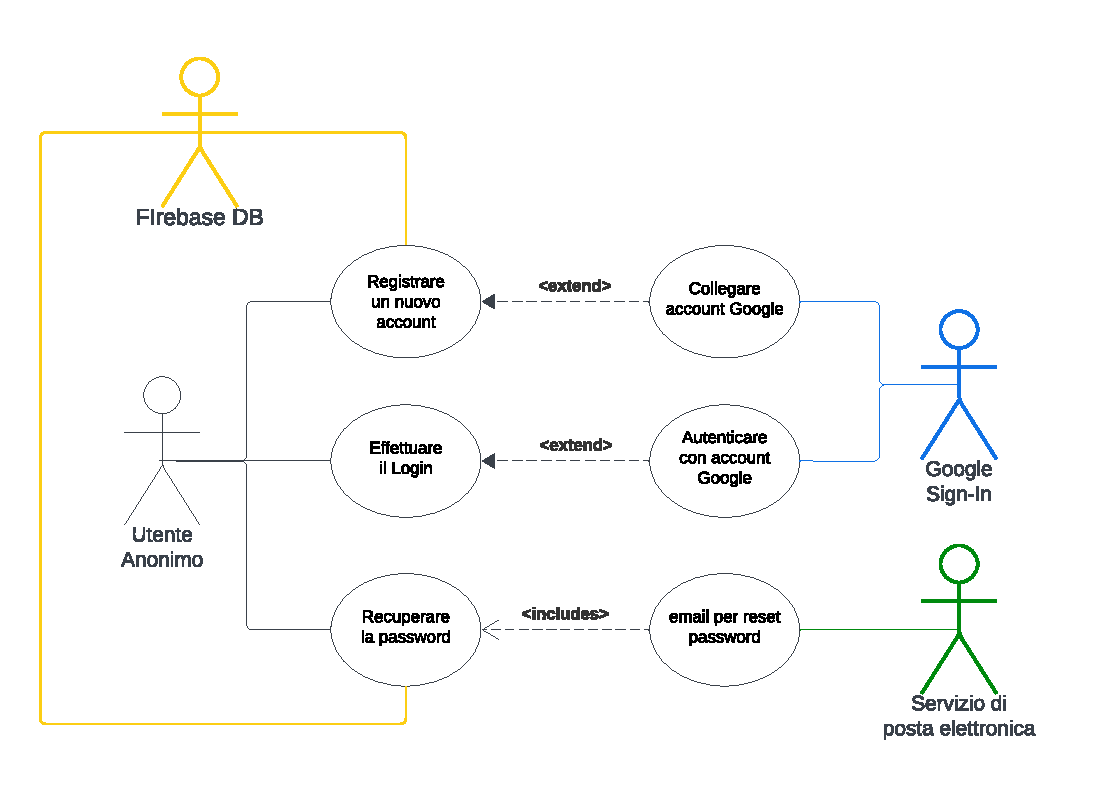
\includegraphics[scale=0.6]{materiale/accesso.pdf}
\caption{UCD dello scenario di accesso al servizio}
\end{figure}

\subsubsection*{Descrizione Use Case \textit{Registrare un nuovo account}}
\subsubsection*{Descrizione Use Case \textit{Recuperare la password}}



\newpage
\subsection{Consultazione dei problemi}
\begin{itemize}
    \item \textbf{RF 4.} Consultazione del catalogo dei problemi
    \item \textbf{RF 5.} Consultazione di un problema
    \item \textbf{RF 9.} Metadati aggiuntivi
    \item \textbf{RF 10.} Progressi
\end{itemize}

\begin{figure}[H]
\centering
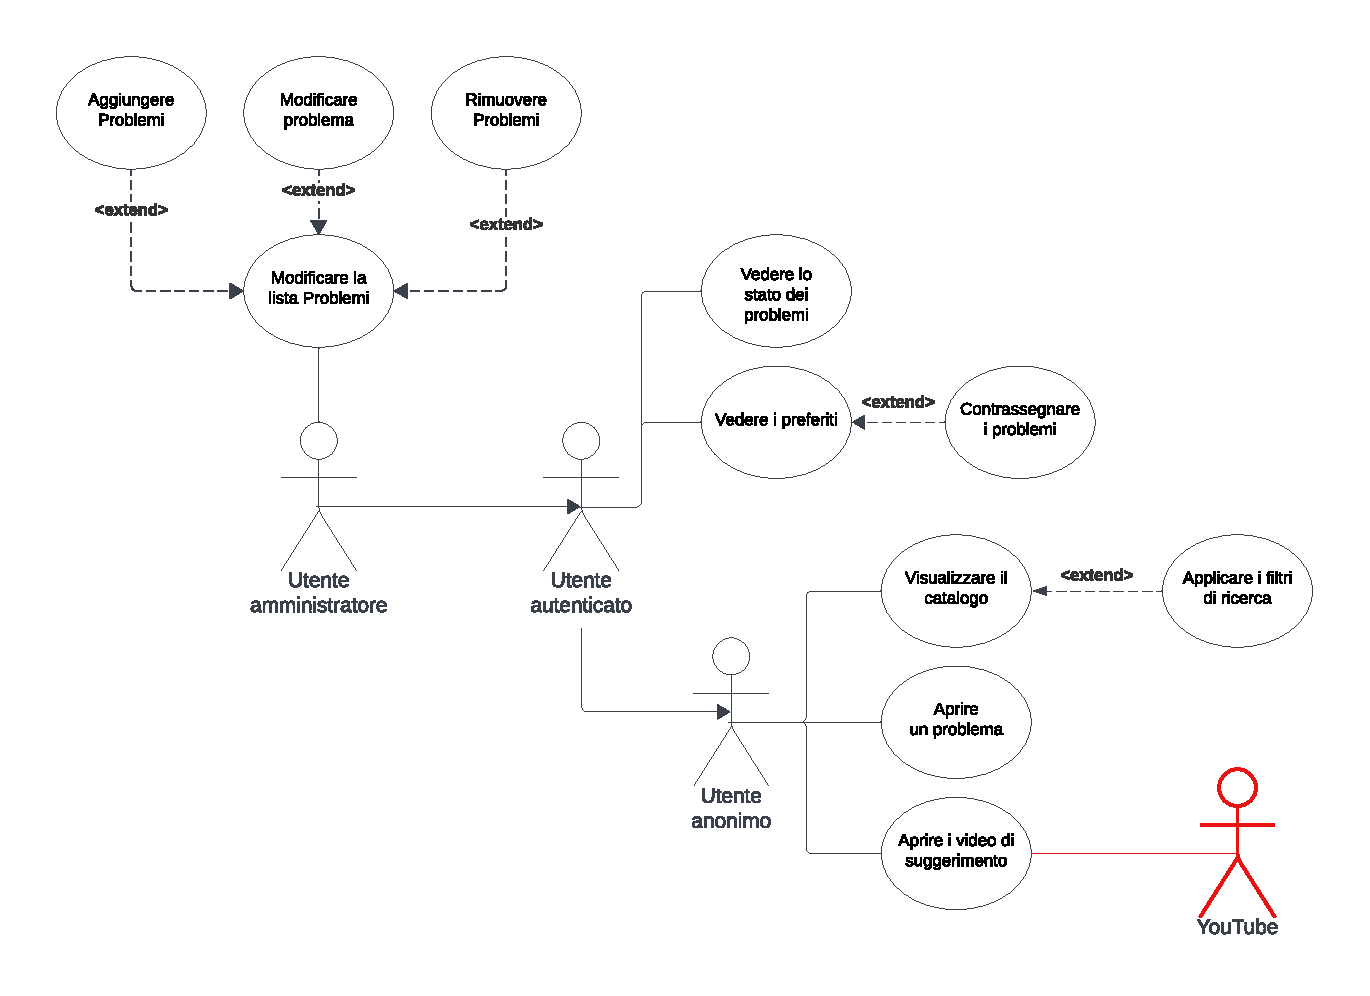
\includegraphics[scale=0.81]{materiale/consulta-catalogo.pdf}
\caption{UCD dello scenario della consultazione dei problemi}
\end{figure}


\newpage
\subsection{Esercitazione}
\begin{itemize}
    \item \textbf{RF 6.} Avviare l'esercitazione
    \item \textbf{RF 7.} Correttezza sintattica del codice
    \item \textbf{RF 8.} Correttezza dell'algoritmo
    \item \textbf{RF 10.} Progressi
\end{itemize}

\begin{figure}[H]
\centering
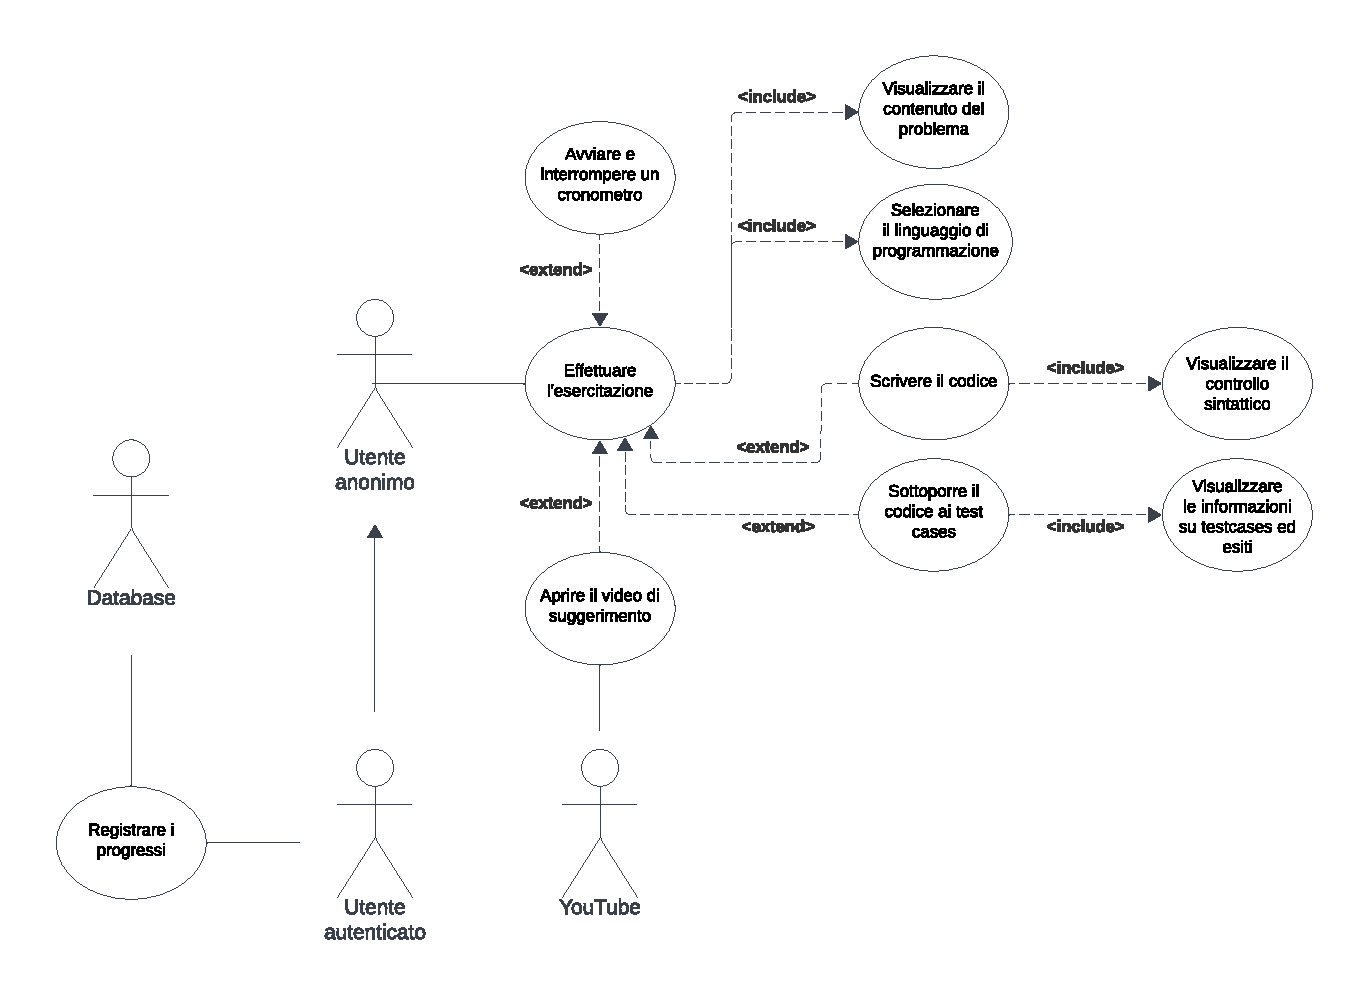
\includegraphics[scale=0.57]{materiale/esercitazione.pdf}
\end{figure}

\subsubsection*{Descrizione Use Case \textit{Registrare i progressi}}

\newpage
\subsection{Gestione del profilo e dell'account}
\begin{itemize}
    \item \textbf{RF 10.} Progressi
    \item \textbf{RF 11.} Aggiornamento dei dati dell'account
    \item \textbf{RF 12.} Logout
\end{itemize}

\begin{figure}[H]
\centering
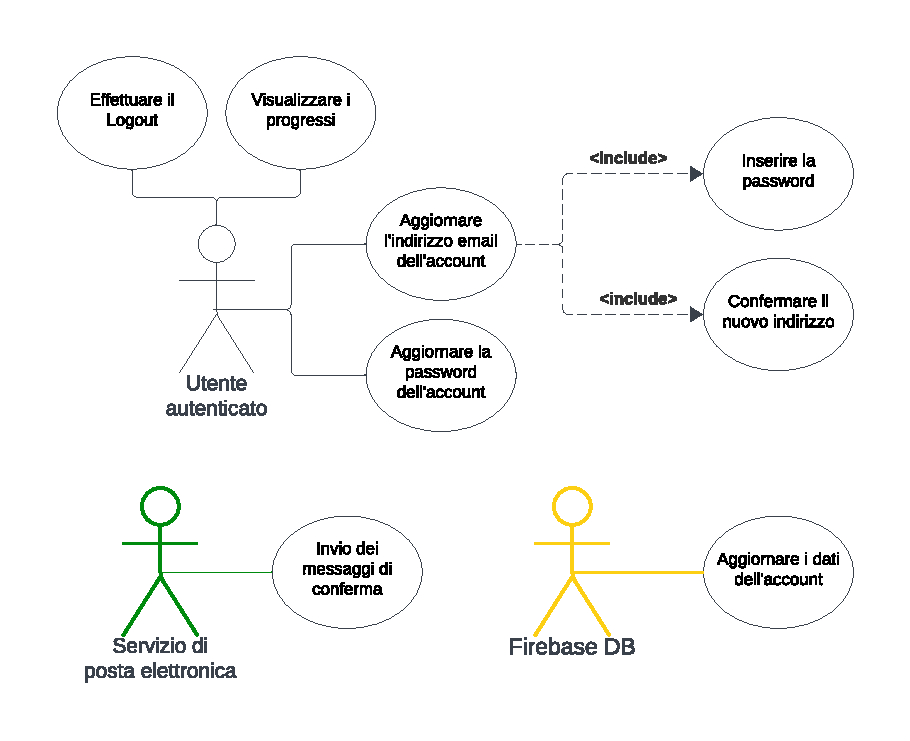
\includegraphics[scale=0.8]{materiale/gestione-account.pdf}
\caption{UCD dello scenario}
\end{figure}

\newpage
\section{Requisiti non funzionali}
Nella presente sezione sono riportati i requisiti non funzionali (RNF)
del sistema utilizzando tabelle strutturate e specificando misure che
consentano di effettuare facilmente delle verifiche quantitative.

\subsection{Caratteristiche di sistema}

\begin{nonfuncreq}
\textbf{Scalabilità }
\begin{center}
    \footnotesize
    \begin{tabularx}{\textwidth}{|X||X||X|}
        \hline
        \cellcolor{red!70}Proprietà & \cellcolor{red!70}Descrizione & \cellcolor{red!70}Misura\\
        \hline
        Elaborazione con un numero crescente di utenti. & Capacità del sistema di gestire un numero crescente di utenti in simultanea. & Viene garantito l'accesso in simultanea di almeno 300 utenti nel primo anno dal lancio.\\
        \hline
        Memorizzazione dei dati degli utenti & Capacità del sistema di gestire i dati generati da un numero crescente di utenti utilizzatori. & Capacità sufficiente per almeno 400 utenti. \\
        \hline
    \end{tabularx}
\end{center}
\end{nonfuncreq}

\begin{nonfuncreq}
    \textbf{Compatibilità }
    \begin{center}
        \footnotesize
        \begin{tabularx}{\textwidth}{|X||X||X|}
            \hline
            \cellcolor{red!70}Proprietà & \cellcolor{red!70}Descrizione & \cellcolor{red!70}Misura\\
            \hline
            Compatibilità client & La piattaforma del servizio deve essere compatibile con e accessibile attraverso le versioni più recenti dei principali browser in commercio. &
            \begin{itemize}
                \item Chrome
                
                117.0.5938.150
                \item Firefox
                
                18.0.1
                \item Edge:
                
                17.0.2045.60
            \end{itemize}La compatibilità deve valere anche per le rispettive versioni superiori.\\
            \hline
        \end{tabularx}
    \end{center}
\end{nonfuncreq}

\begin{nonfuncreq}
    \textbf{Usabilità }
    \begin{center}
        \footnotesize
        \begin{tabularx}{\textwidth}{|X||X||X|}
            \hline
            \cellcolor{red!70}Proprietà & \cellcolor{red!70}Descrizione & \cellcolor{red!70}Misura\\
            \hline
            Usabilità & Intuitività e facilità nell'apprendimento, accesso e impiego delle funzionalità fornite dal servizio. & Il nuovo utente deve poter conoscere e utilizzare il 90\% delle funzionalità (disponibili al proprio livello di accesso) in meno di 30 minuti.\\
            \hline
        \end{tabularx}
    \end{center}
\end{nonfuncreq}

\newpage
\begin{nonfuncreq}
    \textbf{Aspetto }
    \begin{center}
        \footnotesize
        \begin{tabularx}{\textwidth}{|X||X||X|}
            \hline
            \cellcolor{red!70}Proprietà & \cellcolor{red!70}Descrizione & \cellcolor{red!70}Misura\\
            \hline
            Colore & Gamma cromatica dell'interfaccia e distribuzione del colore. La scelta ricade su colori, tinte (aggiunta di bianco) e sfumature (aggiunta di nero) che mirano a limitare l'affaticamento della vista. & Colori caldi; colori freddi presenti in sfumature scure; colori freddi accesi presenti al più in aree ristrette (pulsanti e icone).\\
            \hline
            Contrasto & Accostamento dei colori all'interno dell'interfaccia utente. Mira alla leggibilità e alla limitazione dell'affaticamento della vista. & Regola dei complementari; cerchio di Itten.\\
            \hline
        \end{tabularx}
    \end{center}
\end{nonfuncreq}

\begin{nonfuncreq}
    \textbf{Lingua }
    \begin{center}
        \footnotesize
        \begin{tabularx}{\textwidth}{|X||X||X|}
            \hline
            \cellcolor{red!70}Proprietà & \cellcolor{red!70}Descrizione & \cellcolor{red!70}Misura\\
            \hline
            Lingua di sistema           & Lingua presente nell'interfaccia e nelle risorse fornite dal servizio. & L'interfaccia generale della piattaforma contiene testo in italiano (100\%); i testi dei problemi sono scritti in italiano (100\%); le risorse multimediali (video-suggerimento) devono essere in italiano oppure in inglese.\\
            \hline
        \end{tabularx}
    \end{center}
\end{nonfuncreq}

\begin{nonfuncreq}
    \textbf{Prestazioni }
    \begin{center}
        \footnotesize
        \begin{tabularx}{\textwidth}{|X||X||X|}
            \hline
            \cellcolor{red!70}Proprietà & \cellcolor{red!70}Descrizione & \cellcolor{red!70}Misura\\
            \hline
            Caricamento all'accesso & Tempo massimo richiesto per caricare le pagine rilevanti dopo la ricerca in browser. & Il caricamento delle pagine di login e home (per quest'ultima si considera l'intervallo di tempo che comincia dopo la richiesta di autenticazione) non deve eccedere i 2 secondi.\\
            \hline
            Transizioni & Tempo massimo richiesto per effettuare una transizione da una pagina all'altra.  & Una transizione non deve richiedere più di 2 secondi.\\
            \hline
        \end{tabularx}
    \end{center}
\end{nonfuncreq}


\subsection{Affidabilità}

\begin{nonfuncreq}
    \textbf{Downtime }
    \begin{center}
        \footnotesize
        \begin{tabularx}{\textwidth}{|X||X||X|}
            \hline
            \cellcolor{red!70}Proprietà & \cellcolor{red!70}Descrizione & \cellcolor{red!70}Misura\\
            \hline
            Downtime & Tempo medio massimo in cui il servizio non è raggiungibile; principalmente per motivi di manutenzione e aggiornamento. & 2,7\% (240 ore) nel primo anno 0,85\% (72 ore) dopo il primo anno dal lancio.\\
            \hline
        \end{tabularx}
    \end{center}
\end{nonfuncreq}

\begin{nonfuncreq}
    \textbf{Disponibilità }
    \begin{center}
        \footnotesize
        \begin{tabularx}{\textwidth}{|X||X||X|}
            \hline
            \cellcolor{red!70}Proprietà & \cellcolor{red!70}Descrizione & \cellcolor{red!70}Misura\\
            \hline
            Disponibilità & Probabilità che il sito non si guasti entro un intervallo di tempo trascorso dopo l'entrata in servizio. & Probabilità di resistere ai guasti al 98\% entro le prime 8.000 ore.\\
            \hline
        \end{tabularx}
    \end{center}
\end{nonfuncreq}

\subsection{Privacy e sicurezza}

\begin{nonfuncreq}
    \textbf{Privacy e trattamento dei dati }
    \begin{center}
        \footnotesize
        \begin{tabularx}{\textwidth}{|X||X||X|}
            \hline
            \cellcolor{red!70}Proprietà & \cellcolor{red!70}Descrizione & \cellcolor{red!70}Misura\\
            \hline
            Normativa & Conformità con le vigenti norme relative al trattamento e alla protezione dei dati (GDPR). In particolare, i dati personali dell'utente registrato (nome, email e password) non devono essere divulgati in alcun modo e, qualora lo ritenga opportuno, l'utente ha il diritto di richiedere l'eliminazione delle proprie informazioni dal servizio al fine di interrompere il trattamento. & Conformità del servizio e funzionalità a supporto dell'utente (eliminazione account).\\
            \hline
        \end{tabularx}
    \end{center}
\end{nonfuncreq}

\begin{nonfuncreq}
    \textbf{Connessione sicura }
    \begin{center}
        \footnotesize
        \begin{tabularx}{\textwidth}{|X||X||X|}
            \hline
            \cellcolor{red!70}Proprietà & \cellcolor{red!70}Descrizione & \cellcolor{red!70}Misura\\
            \hline
            Connessione sicura & Impiego di protocolli di comunicazione che garantiscono la confidenzialità e riservatezza delle informazioni scambiate tra client e server. & Utilizzo del protocollo \texttt{https}.\\
            \hline
        \end{tabularx}
    \end{center}
\end{nonfuncreq}

\begin{nonfuncreq}
    \textbf{Password strength }
    \begin{center}
        \footnotesize
        \begin{tabularx}{\textwidth}{|X||X||X|}
            \hline
            \cellcolor{red!70}Proprietà & \cellcolor{red!70}Descrizione & \cellcolor{red!70}Misura\\
            \hline
            Password sicura & Quantità e varietà di caratteri necessari per comporre una password forte. & Una password conforme possiede da 8 a 64 caratteri, tra i quali sono presenti almeno: una lettera maiuscola, una minuscola, una cifra decimale e un carattere speciale tra ! ? \# \$ \% \& @ * + - / $\backslash$ = \_ . , ; : ( ) [ ] \{ \}.\\
            \hline
        \end{tabularx}
    \end{center}
\end{nonfuncreq}






\newpage
\section{Analisi del contesto}
% riguarda il backend e i componenti esterni al sistema: tutto il codice che utilizzate ma che non avete scritto voi
% flusso di informazioni tra il nostro sistema e quelli esterni

\subsection{Utenti e sistemi esterni} % chi interagisce, chi usa e chi supporta (sia software che umano)
\subsubsection{User}
\subsubsection{Database}
\subsubsection{...}


\subsection{Diagramma di contesto} % frecce = dati che si scambiano. Utente --atuenticaz--> sistema (è l'utente che fornisce i dati al sistema; la freccia indica il verso del flusso)

% INVIO DI EMAIL per recupero password
% freccia da utente a sistema: richiesta recupero password
% freccia da sistema a utente: form
% freccia da utente a sistema: email nuova
% (di mezzo potrebbe essere meglio mettere il database che verifica l'email)
% freccia da sistema a servizio mail: INDIRIZZO MAIL untente, mittente, oggetto, testo, allegati (contenuto in generale) incluso LINK AL FORM DELLA PIATTAFORMA PER IL RESET PASSWORD

% 







\newpage
\section{Analisi dei componenti}

\end{document}